\documentclass[main.tex]{subfiles}
\begin{document}


\chapter{Mehrdimensionale Differentialrechnung}


Sei $U \in \R^n$ offen, $f: U \to \R^m, m,n \geq 1$ und sei $||.||$ die euklidische Norm.


\section{Die Ableitung und Ableitungsregeln}

\begin{Definition}[Differenzierbarkeit]
  Die Funktion $f: U \to \R^m$ heißt bei $x_0 \in U$ \textbf{differenzierbar}, falls eine lineare Abbildung $L:\R^n \to \R^m$ existiert, so dass
  $$\lim \limits_{n \to 0} \dfrac{||f(x_0 + h) - f(x_0) - L(h)||}{||h||} = 0$$
  In diesem Fall heißt $L$ die \textbf{totale Ableitung} von $f$ an der Stelle $x_0$. Wir schreiben
  $$L = (Df)(x_0)$$
  $f$ heißt (in $U$) differenzierbar, falls $f$ bei jedem $x_0 \in U$ differenzierbar ist.
\end{Definition}

\begin{Bemerkung}
  \begin{itemize}
    \item Die Ableitung $Df$ nennt man auch Differential oder Tangentialabbildung.
    \item $L$ ist durch die obige Bedingung eindeutig bestimmt.
    \item $f$ differenzierbar $\Rightarrow$ $f$ stetig
    \item Die Ableitung von $f: U \subseteq \R \to \R$ ist ein Sonderfall mit $L(h) \in \R$:
      $$f'(x_0) = \lim \limits_{n \to 0} \dfrac{f(x_0 + h) - f(x_0)}{h} \in \R$$
      Es gilt dann: $L:\R \to \R, L(h) = f'(x_0)\cdot h$ (um wieder die allgemeine Bedingung mit $= 0$ zu erhalten)
    \item Beachte, dass $(Df)(x_0)$ jetzt eine lineare Abbildung $\R^n \to \R^m$ ist (und nicht mehr nur ein numerischer Wert). Wir schreiben zum Beispiel
      $$Df(\underbrace{x_0}_{\in \R^n})(\underbrace{h}_{\in \R^n \text{ beliebig}}) \in \R^m$$
      Genauso gilt: $Df : U \to Hom(\R^n,\R^m)$, $x \mapsto$ ein bestimmter Homomorphismus.

      Das bedeutet, $Df(x)$ kann als Matrix dargestellt werden:
      $$F = (f)_{ji} = (\partial_j \cdot f_i(x))$$
    \item Ist $f$ bei $x_0 \in U$ differenzierbar, so können wir schreiben
      $$f(x_0 + h) = \underbrace{f(x_0) + Df(x_0)(h)}_{\text{affine lineare Funktion}} + R(h)$$
      mit $R(h) := f(x_0 + h) - f(x_0) -Df(x_0)(h)$, einem Restterm, der erfüllt
      $$\lim \limits_{n \to 0} \dfrac{||R(h)||}{||h||} = 0 \text{ also } ||R(h)|| = {\scriptstyle o}(||h||)$$
  \end{itemize}
\end{Bemerkung}

\begin{Definition}[Richtungsableitung]
  Die Ableitung von $f: U \subseteq \R^n \to \R^m$ in Richtung eines Vektors $v \in \R^n$ an der Stelle $x_0 \in U$ ist
  $$(\partial_v f) (x_0) = \lim \limits_{s \to 0} \dfrac{f(x_0+sv)-f(x_0)}{s} \in \R^m \quad s \in \R$$
  falls der Limes existiert.

  Ist $v$ der $j$-te kanonische Basisvektor, so nennt man
  $$(\partial_{e_j}f)(x_0) =: \partial_j f(x_0) =: \partial_{x_j}f(x_0) = \dfrac{\partial f}{\partial x_j}$$
  die \textbf{partielle Ableitung} von $f$ bezüglich der $j$-ten Koordinate.
\end{Definition}

\begin{Beispiel}
  $$f(x,y,z) = x(y^2 + \sin(z))$$
  \begin{itemize}
    \item $\partial_x f(x,y,z) = \partial_1 f(x,y,z) = y^2 +\sin(z)$
    \item $\partial_y f(x,y,z) = \partial_2 f(x,y,z) = 2xy$
    \item $\partial_z f(x,y,z) = \partial_3 f(x,y,z) = x \cdot \cos(z)$
  \end{itemize}
\end{Beispiel}

\begin{Theorem}
  Sei $U \subseteq \R^n$ offen und $f : U \to \R^m$ bei $x_0$ differenzierbar. Dann existiert die Ableitung von $f$ in Richtung $v$ für jedes $v \in \R^n$ und es gilt:
  $$(\partial_v f)(x_0) = (Df)(x_0) \cdot v$$
\end{Theorem}

\begin{Beweis}
  Nach der Definition der Ableitung gilt
  $$f(x_0 + h) = f(x_0) + Df(x_0)(h) + R(h) \quad \text{mit } ||R|| = 0(||h||)$$
  Setze $h = sv$, dann folgt
  $$\begin{aligned}
    (\partial_v f)(x_0) & = \lim \limits_{s \to 0} \dfrac{f(x_0 + sv) - f(x_0)}{s} \\
    & = \lim \limits_{s \to 0} \dfrac{(Df)(x_0)(sv) + R(sv)}{s} \\
    & = Df(x_0)(v) + \lim \limits_{s \to 0} \dfrac{R(sv)}{s} \\
    & = Df(x_0)(v)
  \end{aligned}$$
\end{Beweis}

\begin{Bemerkung}
  Insbesondere ist die Matrix der linearen Abbildung $(Df)(x_0): \R^n \to \R^m$ bezüglich der kanonischen Basen gegeben durch:
  $$\left(\begin{array}{c c c c}
    | & | & & | \\
    \partial_1 f(x_0) & \partial_2 f(x_0) & ... & \partial_n f(x_0) \\
    | & | & & |
  \end{array}\right)
  \stackrel{*}{=}
  \left(\begin{array}{c c c c}
    \partial_1 f_1(x_0) & \partial_2 f_1(x_0) & ... & \partial_n f_1(x_0) \\
    \partial_1 f_2(x_0) & \ddots & & \vdots \\
    \vdots & & \ddots & \vdots \\
    \partial_1 f_m(x_0) & \partial_2 f_m(x_0) & ... & \partial_n f_m(x_0)
  \end{array}\right)$$
  $*: f = \left(\begin{array}{c}f_1\\f_2\\ \vdots \\f_m\end{array}\right)$
  Diese Matrix nennt man \textbf{Jakobi-Matrix} von $f$ bei $x_0$.

  Spezialfall: $m=1$, $U \subseteq \R^n$. $f$ wird zu $f: \R^n \to \R$ und differenzierbar. Schreibe
  $$grad \, f(x) = \nabla f(x) = \left(\frac{\partial f}{\partial x_1}, ...,  \frac{\partial f}{\partial x_n}\right)$$
  Also ist
  $$\begin{aligned}
    Df(x)(v) & = \frac{\partial f}{\partial x_1} (x) \cdot v_1 + ... + \frac{\partial f}{\partial x_n} (x) \cdot v_n \\
    & = < grad \, f(x), v > \, \stackrel{CS}{\leq} \, ||grad \, f(x)|| \cdot ||v||
  \end{aligned}$$
  Es herrscht Gleichheit, falls $v = \lambda \cdot grad \, f(x)$ für ein $\lambda > 0$. Der 'Größte Anstieg' von $f$ ist in Richtung $grad \, f(x)$.
\end{Bemerkung}

\begin{Beispiel}[$f:\R^3 \to \R$]
    $$f: \R^3 \to \R \quad f(x_1,x_2,x_3) = x_1 \cdot x_2^2 + \sin(x_3)$$
    Berechne die Ableitung bei $x_0 = (1,-2,3)$.
    \begin{itemize}
      \item $\partial_1 f(x) = \dfrac{\partial f((x_1,x_2,x_3))}{\partial x_1} = x_2^2 \Rightarrow \partial_1 f(x_0) = 4$
      \item $\partial_2 f(x) = \dfrac{\partial f((x_1,x_2,x_3))}{\partial x_2} = 2x_1 \cdot x_2 \Rightarrow \partial_2 f(x_0) = 2 \cdot 1 \cdot (-2) = -4$
      \item $\partial_3 f(x) = \dfrac{\partial f((x_1,x_2,x_3))}{\partial x_3} = \cos(x_3) \Rightarrow \partial_3 f(x_0) = \cos(3)$
    \end{itemize}
    $$\Rightarrow Df(x_0) = (4 \quad -4 \quad \cos(3)) \in M(1 \times 3, \R)$$
\end{Beispiel}

\begin{Beispiel}[$f:\R^2\to\R^3$]
  $$g:\R^2 \to \R^3 \quad g\left(\begin{array}{c}
    x_1 \\ x_2
  \end{array}\right) = \left(\begin{array}{c}
    x_1 \cdot x_2 \\
    x_1 - 3x_2^3 \\
    3 x_1 \cdot x_2^2
  \end{array}\right)$$
  Berechne die Ableitung bei $x_0 = (1,1)$
  \begin{itemize}
    \item $g_1(x) = x_1 \cdot x_2$, also $Dg_1(x) = (x_2, x_1) \Rightarrow Dg_1(x_0) = (1,1)$
    \item $g_2(x) = x_1 - 3x_2^3$, also $Dg_2(x) = (x_1, 9x_2^2) \Rightarrow Dg_2(x_0) = (1,-9)$
    \item $g_3(x) = (3 x_2^2, 6 x_1 \cdot x_2^2)$, also $Dg_3(x) = 6x_1 x_2 \Rightarrow Dg_3(x_0) = (3,6)$
  \end{itemize}
  $$\Rightarrow Dg(x_0) = \left(\begin{array}{c c}
    1 & 1 \\
    1 & -9 \\
    3 & 6
  \end{array}\right)$$
\end{Beispiel}

\begin{Lemma}
  Sei
  $$f= \left(\begin{array}{c} f_1\\ \vdots \\f_n \end{array}\right): U \subseteq \R^n \text{ (offen) }\to \R^m$$
  Es bezeichne$\pi_j: \R^m \to \R$ die Projektion auf die $j$-te Komponente.
  $f$ ist bei $x_0 \in U$ differenzierbar genau dann, wenn die Komponente $f_j = \pi_j \circ f$ für jedes $j = 1, ..., m$ bei $x_0$ differenzierbar ist.

  Dann gilt:
  $$\pi_j \circ Df(x_0) = D (\pi_j \circ f) (x_0)$$
\end{Lemma}

\begin{Beweis}
  Angenommen $f_j := \pi_j \circ f$ ist für jedes $j$ bei $x_0$ differenzierbar. Es giht also eine lineare Funktion $L_j : \R^n \to \R$ und einen Resterm $R_j: \R^n \to \R$ mit
  $$f_j(x_0 + h) = f_j(x_0) + L_j(h) + R_j(h)$$
  (es gilt $R_j = o(||x||)$ für $x \to 0$). Wir können dann schreiben
  $$f(x_0 + h) = \begin{pmatrix}
    f_1(x_0 + h) \\ \vdots \\ f_m(x_0 + h)
  \end{pmatrix} = \begin{pmatrix}
    f_1(x_0) \\ \vdots \\ f_m(x_0)
  \end{pmatrix} + \begin{pmatrix}
    L_1(h) \\ \vdots \\ L_m(h)
  \end{pmatrix} + \begin{pmatrix}
    R_1(h) \\ \vdots \\ R_m(h)
  \end{pmatrix}$$
  Es filt also auch global
  $$f(x_0 + h) = f(x_0) + L(h) + R(h)$$
  In diesem Ausdruck ist $L$ weiterhin linear und es ist wieder $R_j = o(||x||)$ für $x \to 0$. Also ist $f$ differenzierbar und die zu zeigende Formel gilt sofort.

  Ist umgekehrt $f$ bei $x_0$ differenzierbar, so gilt die Formel wieder über selbige Rechnung.
\end{Beweis}

\begin{Theorem}
  Sei $U \subseteq \R^n$ offen, $f: U \to \R^m$. Falls für jedes $j = 1, ..., n$ die partielle Ableitung
  $$\partial_j f = \left(\begin{array}{c} \partial_j f_1\\ \vdots \\ \partial_j f_m \end{array}\right)$$
  auf ganz $U$ existiert \textbf{und} stetig ist, so ist $f$ auf ganz $U$ differenzierbar.
\end{Theorem}

\begin{Beweis}
  Wegen des Lemmas können wir oBda. $m = 1$ annehmen.

  Außerdem können wir (ebenfalls oBdA.) annehmen, dass $0 \in U$ und wir Differenzierbarkeit bei $x_0 = 0$ zeigen wollen. Ferner können wir oBdA. annehmen, dass $f(x_0) = 0$. Dann gilt für \underline{kleine} $x = \left(\begin{array}{c} x_1 \\ \vdots \\x_n \end{array}\right) \in U$:
  $$\begin{aligned}
    f(x) & = f(x_1, ..., x_n)\\
    & = f(x_1,...,x_n) - f(0, x_2, ..., x_n) \\
    & + f(0, x_2,...,x_n) - f(0, 0, x_3, ..., x_n) \\
    & \vdots \\
    & + f(0,...,0,x_n) - f(0, 0, ..., 0) \\
  \end{aligned}$$
  Die Funktion $k: [0,x_j] \to \R$ durch $k(t) = f(0,...,0,x_j,x_{j+1},...,x_n)$ ist nach Hyptothese stetig differenzierbar: Die Ableitung entsorucht gerade der $j$-ten partiellen Ableitung von $f$. Nach dem Mittelwertsatz existiert also ein Zwischenpunkt $\xi_j \in [0,x_j]$ so, dass
  $$\partial_j f(0,...,0,\xi_j,x_{j+1},...,x_n) = f(0,...,0,x_j,x_{j+1},...,x_n) - f(0,...,0,0,x_{j+1},...,x_n)$$
  Für eine beliebige Wahl solcher Zwischenpunkte $\xi_j$ haben wir dann
  $$\begin{aligned}
  f & = \partial_1 f(\xi_1,x_2,x_3,...,x_n) \cdot x_1 \\
  & + \partial_2 f(0,\xi_2,x_3,...,x_n) \cdot x_2 \\
  & + ... \\
  & + \partial_n f(0,0,0,...,\xi_n) \cdot x_n
  \end{aligned}$$
  Wir wollen nun zeigen, dass $L: (v_1,...,v_n) \mapsto \partial_1 f(0) \cdot v_1 + ... + \partial_n f(0) \cdot v_n$ der Ableitung $Df(0)$ entspricht. Hierfür schätzen wir ab:
  $$\begin{aligned}
    R(x) & := f(x) - L(x) \\
    & = f(0 + x) -f(0) - L(x) \\
    & = (\partial_1 f(\xi_1, x_2, x_3, ..., x_n) - \partial_1 f(0)) \cdot x_1 \\
    & + (\partial_2 f(0, \xi_2, x_3, ..., x_n) - \partial_2 f(0)) \cdot x_2 \\
    & + \vdots \\
    & + (\partial_n f(0,0,...,0\xi_n) - \partial_n f(0)) \cdot x_n \\
  \end{aligned}$$
  Nach Annahmen und weil $\frac{|x_j|}{||x||} < \leq 1$ für alle $x \in \R^n$ gilt
  $$\lim{x \to 0} \dfrac{R(x)}{||x||} = 0$$
  Das bedeutet nun, dass $f$ bei $x_0 = 0$ differenzierbar ist und dass die Ableitung $Df(0) = L$ ist.
\end{Beweis}

\begin{Theorem}[Kettenregel]
  Es seien $n, m, k \geq 1$ und seien $U \subseteq \R^n$ und $V \subseteq \R^m$ offen. Seien $f: U \to V$, $g: V \to \R^k$ Funktionen. Sei $x_0 \in U$.

  Ist $f$ bei $x_0$ differenzierbar und $g$ bei $y_0 = f(x_0)$ differenzierbar, dann ist $g \circ f$ bei $x_0$ differenzierbar und es gilt:
  $$\begin{aligned}
    D f(x_0) : & \R^n \to \R^m  \\
    D g(y_0) : & \R^m \to \R^k \\
    D(g \circ f)(x_0) : & D g (f(x_0)) \circ D f(x_0)
  \end{aligned}$$
\end{Theorem}
\begin{Bemerkung}[Erinnerung]
  \begin{itemize}
    \item Sei $L: \R^n \to \R^m$ eine lineare Abbildung. Schreibe (für die Operator-Norm)
      $$||L||_{op} = \sup \{ \underbrace{||L(v)||}_{ \in \R^m} \mid v \in \R^n \text{ mit } \underbrace{||v||}_{ \in \R^n} = 1 \}$$
      Diese existiert nach Heine-Borel. ($L(v)$ ist stetig und $||v||=1$ stellt eine abgeschlossene, beschränkte Teilmenge dar.) Es gilt
      $$||L(v)|| \leq ||L||_{op} \cdot ||v|| \A v \in \R^n$$
    \item Landau-Notation:
    $$x = o(y) \Leftrightarrow \limx \dfrac{x}{y} = 0$$
  \end{itemize}

\end{Bemerkung}
\begin{Beweis}
 Es gilt
 $$f(x_0 + x) = f(x_0) + L(x) + R(x) \qquad L = D f(x_0) \quad \underbrace{R(x) = {\scriptstyle o}(||x||)}_{\text{für } x \to 0}$$
 $$g(y_0 + y) = g(y_0) + M(y) + S(y) \qquad M = D y (y_0) \quad S(y) = {\scriptstyle o}(||y||)$$
 Definiere nun: $y:= f(x_0 + x) - f(x_0) = L(x) + R(x)$. Nun gilt
 $$\begin{aligned}
   g(f(x_0 + x)) & = g(y_0 + y) \\
   & = g(y_0) + M(y) + S(y) \\
   & = g(f(x_0)) + \underbrace{M(L(x)) + M(R(x))}_{\text{aufgeteilt weil $M$ linear ist}} + S(L(x) + R(x))
 \end{aligned}$$
 Behauptung: $T(x) = M(R(x)) + S(L(x) + R(x))$.

 Wir müssen also zeigen: $T(x) = o(||x||)$.
 $$||M(R(x))|| \leq ||M||_{op} \cdot ||\underbrace{R(x)}_{o(||x||)}|| = o(||x||)$$

 Zweiter Term: $S(y) = o(||y||)$ bedeutet $\A \varepsilon > 0 \E \delta > 0$ mit
 $$||y|| < \delta \Rightarrow ||S(y)|| < \varepsilon ||y||$$
 Für $y = L(x) + R(x)$:
 $$\begin{aligned}
   ||y|| & \leq ||L(x)|| + ||R(x)|| \\
   & \leq ||L||\cdot ||x|| + o(||x||)
 \end{aligned}$$
 Für $C := ||L|| + 1$ gilt $\E \eta > 0$
 $$||y|| \leq C \cdot ||x|| \quad \text{für } ||x|| \leq \eta$$
 Für $||x|| < \eta$ gilt dann
 $$\begin{aligned}
   ||S(L(x) + R(x))|| & \leq \varepsilon \cdot ||L(x) + R(x)|| \\
   & \leq  C \cdot \varepsilon \cdot ||x|| \\
   & = o(||x||)
 \end{aligned}$$
 $$\Rightarrow T(x) = o(||x||)$$
\end{Beweis}

\begin{Beispiel}
  \begin{itemize}
    \item $n = m = k = 1$.
      $$\begin{aligned}
        f: \R \to \R & \qquad f(x) = x^2 \\
        g: \R \to \R & \qquad g(y) = \sin(y)
      \end{aligned}$$
      Setze $x_0 = 2$.
        $$\begin{aligned}
          Df(x_0): \R & \to \R \\
          1 & \mapsto f'(x_0) = 4 \\
          v & \mapsto 4 v
        \end{aligned}$$
        $$\begin{aligned}
          Dg(y_0): \R & \to \R \\
          1 & \mapsto g'(y_0) = \cos(4) \\
          w & \mapsto \cos(4) \cdot w
        \end{aligned}$$
      Es gilt $g(f(x)) = \sin (x^2)$, folgt:
      $$\begin{aligned}
        D(g \circ f) (x_0) : \R & \to \R \\
        1 & \mapsto 4 \cos(4)
      \end{aligned}$$
      $$M(L(v)) = M(4v) = \cos(4) \cdot 4 v$$
    \item $n = m = k = 2$
      $$\begin{aligned}
        f: \R^2 \to \R^2 & \qquad f(x,y) = (xy + 2 x^2 + \sin(y), 2y) \\
        g: \R^2 \to \R^2 & \qquad g(s,t) = (\exp(s\cdot t),\pi)
      \end{aligned}$$
      Setze $(x_0,y_0) = (0,0)$, also $(s_0, t_0) = f(x_0,y_0) = (0,0)$
        $$\begin{aligned}
          Df(x_0,y_0): \R^2 & \to \R^2 \\
          e_1  = \left(\begin{array}{c} 1 \\ 0 \end{array}\right) & \mapsto \dfrac{\partial f}{\partial x}(x_0,y_0) = \left(\begin{array}{c} 0 \\ 0 \end{array}\right) \\
          e_2  = \left(\begin{array}{c} 0 \\ 1 \end{array}\right) & \mapsto \dfrac{\partial f}{\partial y}(x_0,y_0) = \left(\begin{array}{c} 1 \\ 2 \end{array}\right) \\
          v & \mapsto \left(\begin{array}{c c} 0 & 1 \\ 0 & 2 \end{array}\right) \cdot v
        \end{aligned}$$
        $$\begin{aligned}
          Dg(s_0,t_0): \R^2 & \to \R^2 \\
          e_1  = \left(\begin{array}{c} 1 \\ 0 \end{array}\right) & \mapsto \dfrac{\partial g}{\partial x}(s_0,t_0) = \left(\begin{array}{c} 0 \\ 0 \end{array}\right) \\
          e_2  = \left(\begin{array}{c} 0 \\ 1 \end{array}\right) & \mapsto \dfrac{\partial g}{\partial y}(s_0,t_0) = \left(\begin{array}{c} 0 \\ 0 \end{array}\right) \\
          v & \mapsto \left(\begin{array}{c c} 0 & 0 \\ 0 & 0 \end{array}\right) \cdot v
        \end{aligned}$$
      Nur $0$ an der Stelle $(s_0,t_0)$.
    \item Sei $\mathcal{I} \subseteq \R$ ein offenes Intervall, $U \subseteq \R^n$ und $g: U \to \R^m$ differenzierbar.
      In dem Fall gilt für $t_0 \in \mathcal{I}$
      $$\begin{aligned}
        Df(t_0): \R & \to \R^n \\
        1 & \mapsto (f_1'(t_0), ..., f_n'(t_0)) = f'(t_0)
      \end{aligned}$$
      $$Dg(x_0): \R^n \to \R^m$$
      Für $x_0 = f(t_0)$ kann man jetzt schreiben
      $$D(g \circ f)(t_0) = Dg (x_0)\circ f(t_0)$$
      $$D(g \circ f)(t_0)(1) = Dg(x_0)(Df(t_0)(1)) = Dg (x_0) (f'(t_0))$$
      \textbf{Konkretes Beispiel:}
      $$\begin{aligned}
        \gamma: \R \to \R^2 & \qquad \gamma(t) = (t,t^2) \\
        g: \R^2 \to \R^2 & \qquad g(x,y) = (xy,\sin(y))
      \end{aligned}$$
  \end{itemize}
\end{Beispiel}

\begin{Theorem}[Mittelwertsatz]
  Sei $U \subseteq \R^n$ offen, $f: U \to \R$ differenzierbar, $x_0 \in U$, $h \in \R^n$ mit $x_0 + t\cdot h \in U$ für alle $t \in [0,1]$. Dann existiert ein $t_0 \in (0,1)$ mit
  $$f(x_0 + h) - f(x_0) = Df(\xi_0)(h) \qquad \xi_0 = x_0 +t_0 \cdot h$$
\end{Theorem}

\begin{Beweis}
  Betrachte $\gamma: [0,1] \to \R$ gegen durch $\gamma(t) = f(x_0 + t\cdot h)$. Die Funktion $\gamma$ ist differenzierbar auf $(0,1)$ also insbesondere stetig. Hier gilt der bekannte, 1-dimensionale Mittelwertsatz:
  $$\E t_0 \in (0,1): \gamma(1) - \gamma(0) = \gamma'(t_0)$$
  $$\begin{aligned}
    & \Leftrightarrow & f(x_0 + h - f(x_0)) & = D\gamma(t_0)(1) \\
    & & & = Df(x_0 + t_0 \cdot h) \cdot (Dg(t_0)(1)) \\
    & & & = Df(\xi_0)(h)
  \end{aligned}$$
  ($g(t):= x_0 + th$)
\end{Beweis}

\begin{Korollar}
  Sei $U \subseteq \R^n$ offen und ammenhängend und sei $f: U \to \R$ differenzierbar.
  $$Df(x) = 0 \A x \in U\Leftrightarrow f \text{ ist konstant}$$
\end{Korollar}

\begin{Beweis}
  Wähle $x_0 \in U$ und setze
  $$U' = \{x \in U \mid f(x) = f(x_0) \} \subseteq U$$
  Zeige $U'$ offen und abgeschlossen $\Rightarrow$ $U' = U$.

  $U'$ ist abgeschlossen: Denn $f$ ist stetig.

  $U'$ ist offen: Sei $x \in U'$. Da $U \subseteq \R^n$ offen ist, existiert $r > 0$ mit $B(x,r) \subseteq U$. Sei $y = x+h$ ein Element von $B(x,r)$. Nach dem Mittelwertsatz existiert $\xi_0 = x + t_0 \cdot h$ mit
  $$f(y) - f(x) = \underbrace{Df(\xi_0)(h)}_{=0} \Rightarrow f(y) = f(x) \Rightarrow y \in U'$$
  Folgt $U' \subseteq U$ offen und abgeschlossen und nicht leer, also $U' = U$.
\end{Beweis}

\begin{Definition}[Lokale Lipschitz-Stetigkeit]
  Sei $U \subseteq \R^n$, $f: U \to \R^n$. Wir sagen $f$ sei \textbf{lokal Lipschitz}, falls für jeden Punkt $x_0 \in U$ eine offene Umgebung $U_0$ von $x_0$ existiert, so dass $f |_{U_0}$ Lipschitz-stetig ist.
\end{Definition}

\begin{Beispiel}
  Jede stetig differenzierbare Funktion in einer Variable ist lokal Lipschitz.

  Als Gegenbeispiel ist $f(x) = \sqrt{|x|}$.
\end{Beispiel}

\begin{Theorem}
  Sei $U \subseteq \R^n$ offen, $f: U \to \R^n$ stetig differenzierbar. Dann
  \begin{enumerate}
    \item ... ist $f$ lokal Lipschitz.
    \item ..., falls $Df$ beschränkt und $U$ konvex ist, dann ist $f$ Lipschitz.
  \end{enumerate}
\end{Theorem}

\begin{Beweis}
  Aussage $(2)$:

  Dass $Df$ beschränkt ist, bedeutet
  $$\E M \in \R: ||Df(x)||_{op} \leq M \A x \in U$$
  (Die Operator-Norm ist stellvertretend gewählt, denn auf einem endlich-dimensionalen $\R$-Vektorraum, wie dem der Homomorphismen, sind alle Normen äquivalent)

  Es gilt dann für alle $x,y \in U$:
  $$x + t \cdot (y - x) \in U \A t \in [0,1]$$
  da $U$ konvex ist. Dank dem Mittelwertsatz gilt folgende Aussage
  $$\begin{aligned}
    & & f(y) - f(x) & = Df(\xi_0)(y-h) \\
    & \Leftrightarrow & ||f(y) - f(x)|| & = ||Df(\xi_0)(y-h)|| \\
    & & & \leq M \cdot ||y - x||
  \end{aligned}$$
  Folgt $f$ ist Lipschitz mit Konstante $M$.

  Aussage $(1)$:

  Bemerke: Zu $x \in U \E r > 0 : \overline{B(x,r)} \subseteq U$. Der abgeschlossene Ball $\overline{B(x,r)}$ ist kompakt (weil beschränkt). Setze
  $$M = \max \{||Df(y)||_{op} \mid y \in \overline{B(x,r)} \}$$
  (wohldefiniert, dank Heine-Borel)
  $$\Rightarrow f|_{B(x,r)} : B(x,r) \to \R \text{ ist Lipschitz mit Konstante } M$$
\end{Beweis}


\section{Höhere Ableitungen und Tailor-Approximation}

Vorbedingungen: $U \subseteq \R^n$ offen, $f: U \to \R^m$ stetig differenzierbar.
$$Df : U \to Hom(\R^n,\R^m) (\sim \R^{n\cdot m})$$
falls $Df$ differenzierbar ist, so ist
$$D(Df) : U \to Hom(\R^n,Hom(\R^n,\R^m))$$

Der Vektorraum $ Hom(\R^n,Hom(\R^n,\R^m))$ (mit Dimension $n^2 \cdot m$) ist der Vektorraum aller Bilinearen Abbildungen $\R^n \times \R^n \to \R^m$

\begin{Bemerkung}[allgemein]
  $$Hom(V, Hom(V,W)) = Bil^*(V \times V, W) \qquad V,W \text{ Vektorräume}$$
  $^*$: 2 Variablen, linear für jede Variable, wenn die andere festgehalten wird.
\end{Bemerkung}

$$D(Df) = D^2f: U \to Bil(\R^n \times \R^n, \R^m)$$
$$\vdots$$
$$D^nf : U \to n-lin(\R^n\times ... \times \R^n,\R^m)$$

\begin{Definition}[Klassen stetig differenzierbarer Funktionen]
  Sei $U \subseteq \R^n$ offen, $f:\R^n \to \R^m$ stetig. Sei $d \geq 0$. Wir sagen $f$ sei von Klasse $C^d$ falls für alle $i_1, i_2,...,i_d \in \{1,2,...,n\}$
  $$\partial_{i_d} ... \partial_{i_2} \partial_{i_1}f(x)$$
  existiert und stetig als Funktion von $x$ ist.

  Schreibe $C^d(U,\R^m)$ für den Vektorraum aller Funktionen $f: U \to \R^m$ von Klase $d$.

  Glatte Funktionen erfüllen:
  $$\bigcap_{d = 0}^\infty C^d(U,\R^m) =: C^\infty (U,\R^m)$$
\end{Definition}

\begin{Theorem}[Satz von Schwarz]
  Sei $U \subseteq \R^n$ offen, $f \in C^d(U, \R^m)$. Dann gilt
  $$\partial_j \partial_k f(x) = \partial_k \partial_j f(x)$$
  $\A x \in U, \A j,k \in \{1,2,...,n\}$.
\end{Theorem}

\begin{Bemerkung}
  Die Aussage gilt nur unter Voraussetzung der Stetigkeit an beide Ableitungen.
\end{Bemerkung}

\begin{Beispiel}[$2$-fache Ableitung einer reellwertigen Funktion in 2 Variablen]
  $$f: \R^2 \to \R \quad f(x,y) = e^{x^2 + y^2}$$
  $$\begin{aligned}
    Df(x,y): \R^2 & \to \R \\
    \left(\begin{array}{c}v_1 \\ v_2 \end{array}\right) & \mapsto 2xe^{x^2 + y^2}v_1 + 2ye^{x^2 + y^2}v_2
  \end{aligned}$$
  oder anders dargestellt:
  $$\nabla f(x,y) = \left(2xe^{x^2 + y^2}, 2ye^{x^2 + y^2}\right)$$
  Jetzt gilt für die 2. Ableitung
  $$\begin{aligned}
    D(\nabla f)(x,y): \R^2 & \to Hom(\R^2,\R) \sim \R^2 \\
    \left( \begin{array}{c} v_1 \\ v_2 \end{array} \right) & \mapsto \left(\begin{array}{c c }2e^{x^2 + y^2} + 4x^2 e^{x^2 + y^2} & 4xy e^{x^2 + y^2}\\ 4xy e^{x^2 + y^2} & 2e^{x^2 + y^2} + 4x^2 e^{x^2 + y^2} \end{array}\right)
  \end{aligned}$$
\end{Beispiel}

\begin{Beweis}
  ObdA. können wir annehmen
  $$n = 2 \quad m=1 \quad k = 1 \quad j = 2$$
  (betrachte einfach eine Funktion, die auf Untermengen eingeschränkt wurde)
  Fixiere $x \in U$ und $h \in \R^+$ klein genug:
  \incfig{satz_von_schwarz1}
  $$F(h) = f(x_1 + h, x_2 + h) - f(x_1, x_2 + h) - f(x_1 + h, x_2) + f(x_1, x_2)$$
  Betrachte $\varphi(t) = f(x_1+th,x_2+h) - f(x_1+th, x_2)$

  Nach dem Mittelwertsatz gilt: $\E \xi_1 \in (0,1)$ mit
  $$\begin{aligned}
    F(h) & = \varphi(1) - \varphi(0) \\
    & = \varphi'(\xi_1) \\
    & = (\partial_1  f(x + \xi_1 \cdot h, x_2 + h) - \partial_1 f(x_1 + \xi_1 \cdot h, x_2)) \cdot h \\
    & = \psi(1) - \psi(0)
  \end{aligned}$$
  $$\psi(t) = \partial_1 f(x_1 + \xi_1 \cdot h, x_2 + t \cdot h)\cdot h$$
  Es gilt wieder nach dem Mittelwertsatz $\E \xi_2 \in (0,1)$ mit
  $$\begin{aligned}
    F(h) & = \psi(1) - \psi(0)
    & = \psi'(\xi_2)
    & = \partial_2 \partial_1 f(x_1 + \xi_1 \cdot h, x_2 + \xi_2 \cdot h) \cdot h^2
  \end{aligned}$$

  Wir gehen genau gleich in die andere Richtung vor: $\E \eta_1, \eta_2 \in (0,1)$ mit
  $$F(h) = \partial_1 \partial_2 f(x_1 + \eta_1 \cdot h, x_2 + \eta_2 \cdot h) \cdot h^2$$
  Folgt:
  $$\partial_1 \partial_2 f(x_1 + \eta_1 \cdot h, x_2 + \eta_2 \cdot h)  = \partial_2 \partial_1 f(x_1 + \xi_1 \cdot h, x_2 + \xi_2 \cdot h)$$
  Mit $\limh$ folgt:
  $$\partial_1 \partial_2 f(x_1, x_2) = \partial_2 \partial_1 f(x_1, x_2)$$
\end{Beweis}

\begin{Bemerkung}[Reformulierung]
  $$\partial_j \partial_k f(x) = D^2f(x)(e_j, e_k) = D^2f(x)(e_k, e_j) = \partial_k \partial_j f(x)$$
  Mit linearer Algebra folgt allgemein:
  $$ D^2f(x)(v, w) =  D^2f(x)(w, v)$$
  Die Bilineare Abbildung
  $$D^2f(x) : \R^n \times \R^n \to \R^n$$
  ist symmetrisch.
\end{Bemerkung}

Allgemeiner
\begin{Theorem}
  Ist $f \in \mathcal{C}^d(U,\R^m)$ so ist
  $$D^df(x): \underbrace{\R^n \times \R^n \times ... \times \R^n}_{d\text{-Mal}} \to \R^m$$
  ist symmetrisch.
\end{Theorem}

\begin{Theorem}[Taylor-Entwicklung]
  Sei $U \subseteq \R^n$ offen, $f: U \to \R$ von Klasse $C^{d+1}$, $x \in U$, $h \in \R^n$ so, dass $x+t\cdot h \in U \A t \in [0,1]$.
  Dann gilt
  $$f(x+h) = f(x) + \sum \limits_{k=1}^d \dfrac{1}{k!} D^k f(x)(\underbrace{h,h,...,h}_{k\text{-Mal}}) + \int_0^1 \dfrac{(1-t)^d}{d!} D^{d+1}f(x + t\cdot h)(h,...h) dt$$
\end{Theorem}

\begin{Beweis}
  Da $U$ offen ist $\E \delta > 0$ mit $x + t \cdot h \in U \A t \in I = (-\delta,1 + \delta)$. Betrachte
  $$\begin{aligned}
    \varphi: I & \to \R \\
    \varphi(t) & = f(x + t \cdot h)
  \end{aligned}$$
  von Klasse $\mathcal{C}^{d+1}$.

  Schreibe die Taylor-Entwicklung für $\varphi$:
  $$\varphi(1) = \varphi(0) + \sum \limits_{k=1}^d \dfrac{\varphi^{(k)}(0)}{k!} + \int_0^1 \varphi^{(d+1)}(t) \dfrac{(1-t)^d}{d!} dt$$
  \begin{itemize}
    \item $\varphi'(t) = \partial_h f(x + t \cdot h) = Df(x+ t \cdot h)(h)$
    \item $\varphi'(0) = \partial_h f(x) = Df(x)(h)$
    \item $\varphi''(0) = D(Df(x+ t \cdot h)(h))|_{t=0}(h) = D^2f(x)(h,h) = \partial_h \partial_h f(x)$
    \item $\vdots$ Induktion
    \item $\varphi^{(k)} (0) = D^k f(x)(h,h,...,h)$
  \end{itemize}
  Setzt man dies in die Taylor-Entwicklung von $\varphi$ ein, so erhält man die gesuchte Formel aus dem Satz.
\end{Beweis}


\section{Extremwerte}

\begin{Bemerkung}[Erinnerung]
  Ein Punkt $x \in U$ heißt lokales Maximum von $f:U\to \R$, falls $\E r > 0 : f(y) \leq f(x) \A y \in B(x,r)$.

  Ein Punkt $x$ heißt isoliertes lokales Minimum, falls $\E r > 0 : f(y) < f(x) \A x \in B(x,r) \backslash \{x\}$
\end{Bemerkung}

\begin{Theorem}[Extremwert merhdimensionaler Funktionen]
  Sei $U \subseteq \R^n$ offen, $f: U \to \R$ differenzierbar, $x_0 \in U$ ein lokales Maximum von $f$. Dann gilt
  $$Df(x_0) = 0$$
\end{Theorem}

\begin{Beweis}
  Für $t > 0$ klein genug gilt $\left\{\begin{aligned}
    f(x_0) - f(x_0 + t \cdot e_j) & \geq 0 \\
    f(x_0) - f(x_0 - t \cdot e_j) & \geq 0
  \end{aligned} \right\}$. Nach Grenzwertbildung sieht man:
  $$\begin{aligned}
    \partial_j f(x_0) = Df(x_0)(e_j) & = \lim \limits_{\substack{t\to 0 \\ t > 0}} \dfrac{f(x_0) - f(x_0 + t \cdot e_j)}{-t} \leq 0 \\
    & = \lim \limits_{\substack{t\to 0 \\ t > 0}} \dfrac{f(x_0) - f(x_0 - t \cdot e_j)}{t} \geq 0 \\
    & = 0
  \end{aligned}$$
  Für beliebige Basisvektoren $\Rightarrow Df(x_0) = 0$
\end{Beweis}

\begin{Definition}[Hesse-Matrix]
  Sei $f:U \to \R$ von Klasse $\mathcal{C}^2$. Die $\text{Hesse-Matrix}$ von $f$ an der Stelle $x_0 \in U$ ist die $n \times n$-Matrix $H(x_0)$ mit den Einträgen
  $$(h)_{ij}(x_0) = D^2f(x_0)(e_i, e_j) = \partial_i \partial_j f(x_0)$$
\end{Definition}

\begin{Beispiel}
  $$f: \R^2 \to \R \quad f(x,y) = 20 \cdot x \cdot \sin(y) + 2x^2 + 2y^2$$
  \begin{center}
    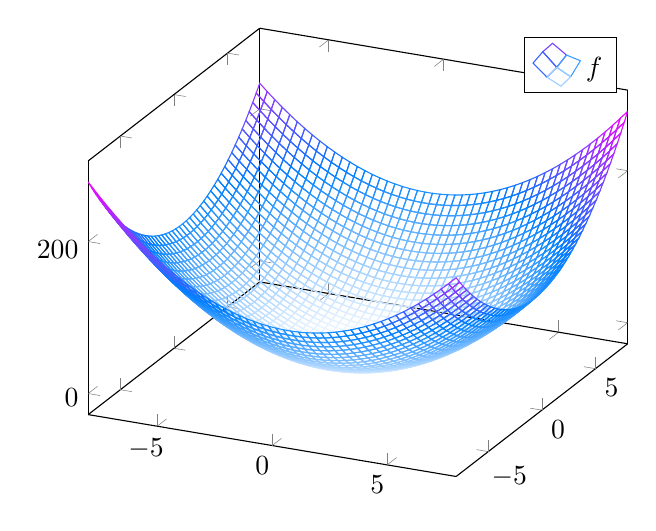
\begin{tikzpicture}
      \begin{axis}[
          % axis lines=center,
          colormap/cool,]
      \addplot3[
          mesh,
          samples=50,
          domain=-8:8,]
      {20 * x * sin(y) + 2*x^2 + 2*y^2};
      \addlegendentry{$f$}
      \end{axis}
    \end{tikzpicture}
  \end{center}
  Berechne nun
  $$H(x_0,y_0) = \left(\begin{array}{c c}
    4 & 20 \cos(y_0)\\
    20\cos(y_0) & -20 \cdot x_0 \cdot \sin(y_0) + 4
  \end{array}\right)$$
  Die bilineare Abbildung $D^2 f(x_0,y_0): \R^2 \times \R^2 \to \R$ ist in $H$ einkodiert.

  Beispielsweise wird
  $$H(0,0) = \left(\begin{array}{c c}
    4 & 20\\
    20 & 4
  \end{array}\right)$$
  Außerdem gilt:
  $$D^2f(x_0,y_0)(v,w) = <v,H(x_0,y_0) \cdot w>$$
\end{Beispiel}

\begin{Definition}[Definitheit]
  Sei $A \in M(n \times n, \R)$ symmetrisch (beispielsweise die Hesse-Matrix).

  Wir sagen $A$ sei \textbf{positiv definit} falls alle Eigenwerte von $A$ positiv sind. (sie sind alle reell, wird in LA gezeigt.)

  Analog ist $A$ \textbf{negativ definit} falls alle Eigenwerte von $A$ negativ sind.

  Ansonsten ist $A$ \textbf{indefinit}.
\end{Definition}

\begin{Theorem}
  Sei $U \subseteq \R^n$ offen, $f \in \mathcal{C}^2 (U,\R^2)$ und $x_0 \in U$ mit $DF(x_0) = 0$. Sei $H(x_0)$ die Hesse Matrix von $f$.
  \begin{itemize}
    \item Ist $H(x_0)$ positiv definit, so ist $x_0$ ein isoliertes Minimum.
    \item Ist $H(x_0)$ negativ definit, so ist $x_0$ ein isoliertes Maximunm.
    \item Ist $H(x_0)$ nicht singuläre (kein Eigenwert ist $=0$) und indefinit, so ist $x_0$ nicht ein lokales Extremum.
  \end{itemize}
\end{Theorem}

\begin{Theorem}
  Sei $U \subseteq \R^n$ offen, $f: U \to \R$ von Klassen $C^2$ und $x_0 \in U$ mit $Df(x_0)= 0$. Sei $H$ die Hesse-Matrix von $f$ bei $x_0$: $h_j = \frac{\partial}{\partial x_i} \frac{\partial}{\partial x_j} f(x_0)$.
  \begin{enumerate}
    \item Ist $H$ positiv definit, so ist $x_0$ ein isoliertes lokales Minimum.
    \item Ist $H$ negativ definit, so ist $x_0$ ein isoliertes lokales Maximum.
    \item Ist $H$ indefinit und nicht sigulär, so ist $x_0$ kein lokales Extremum.
  \end{enumerate}
\end{Theorem}

\begin{Bemerkung}
  Definitheit bedeutet, dass alle Eigenwerte der Matrix $H$ je alle positiv oder negativ sind.
\end{Bemerkung}

\begin{Beweis}
  \begin{enumerate}
    \item $H$ positiv definit $\Leftrightarrow \underbrace{<h,Hh>}_{Q(h)} +> 0 \A h \in \R^n$.

      Achtung: $A(\alpha h) = \alpha^2 Q(h) \A \alpha \in \R \A h \in \R^n$: $Q$ ist eine quadratische Form (also insb. nicht linear)
      \begin{align*}
        f(x_0 + h) - f(x_0) & = \dfrac{1}{2} D^2f(x_0)(h,h) + \mathcal{O}(||h||^3) \\
        & = \dfrac{1}{2} \underbrace{||h||^2}_{Kompensation}\left[ Q\left(\dfrac{h}{||h||}\right) + R(h)\right]
      \end{align*}
      mit $\limh \dfrac{R(h)}{||h||} = 0$
      $Q: S^{n-1} \to \R$ ist stetig, $S^{n-1}$ ist kompakt.
      $$\E c > 0 : Q(v) > c \A v \in S^{n-1} \quad \text{also} \quad Q(h) > c \cdot ||h||^2 \A h \in \R^n\backslash\{0\}$$
      Es existiert $\delta > 0$ mit $\frac{||R(h)||}{||h||} < \frac{c}{2} \A h \in \R^n\backslash\{0\},||h|| < \delta$.
      $$\begin{aligned}
        f(x_0 + h) - f(x_0) & \geq \dfrac{1}{2} ||h||^2 \left(c - \dfrac{c}{2}\right) = \dfrac{c}{4}||h||^2 \\
        & > 0 \text{ für } h \in \R^n\backslash\{0\}, ||h|| < \delta
      \end{aligned}$$
      $$\Leftrightarrow f(x_0 + h) > f(x_0) \Rightarrow x_0 \text{ist eine isoliertes lokales Minimum}$$
    \item Analog
    \item Analog
  \end{enumerate}
\end{Beweis}

\begin{Beispiel}
  $$f: U = \R^2 \to \R \quad (x_0,y_0) = (0,0)$$
  \begin{enumerate}
    \item $f(x,y) = x^2 + y^2$ also $Df(x_0,y_0) = 0$. Allgemein:
      $$Df(x_0,y_0):
      \left\{ \begin{array}{c c c}
        e_1 & \mapsto & \frac{\partial}{\partial x} f(x_0,y_0) = 2 x_0 \\
        e_2 & \mapsto & \frac{\partial}{\partial y} f(x_0,y_0) = 2 y_0
      \end{array} \right\}$$
      $$H = \left(\begin{array}{c c}
        2 & 0 \\
        0 & 2
      \end{array}\right)$$
      ist positiv definit: $<(u,v),H(u,v)> = 2u^2 + 2v^2$.
      \begin{center}
        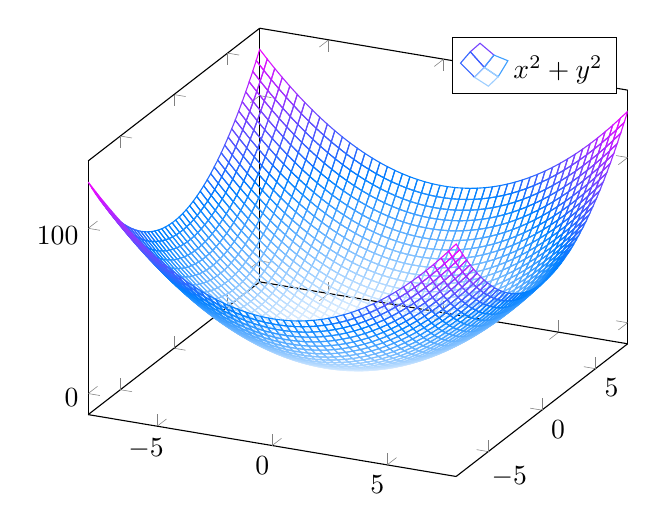
\begin{tikzpicture}
          \begin{axis}[
              % axis lines=center,
              colormap/cool,]
          \addplot3[
              mesh,
              samples=50,
              domain=-8:8,]
          {x^2+y^2};
          \addlegendentry{$x^2+y^2$}
          \end{axis}
        \end{tikzpicture}
      \end{center}
    \item Für $g = -f$ erhält man $H = \begin{pmatrix}
        -2 & 0 \\ 0 & -2
      \end{pmatrix}$
    \item $f(x,y) = x^2 - y^2$, also $H = \left(\begin{array}{c c}
      2 & 0 \\
      0 & -2
    \end{array}\right)$ ist indefinit.
    \begin{center}
      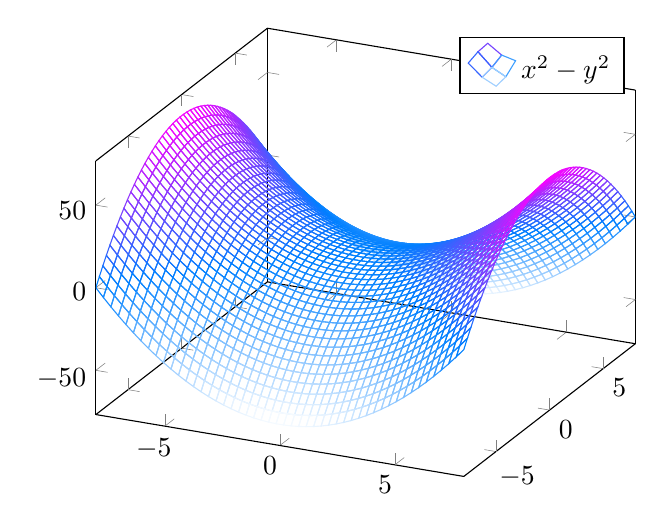
\begin{tikzpicture}
        \begin{axis}[
            % axis lines=center,
            colormap/cool,]
        \addplot3[
            mesh,
            samples=50,
            domain=-8:8,]
        {x^2-y^2};
        \addlegendentry{$x^2-y^2$}
        \end{axis}
      \end{tikzpicture}
    \end{center}
  \end{enumerate}
\end{Beispiel}

\subsection{Zusammenhänge}

$$f(x_0+ h) = \underbrace{f(x_0)}_{konstant} + \underbrace{Df(x_0)(h)}_{linear} + \dfrac{1}{2}\underbrace{D^2f(x_0)(h,h)}_{quadratisch} + ... $$

\begin{Definition}[Totaler Grad]
  Sei $n \geq 1$. Der \textbf{totale Grad} eines Polynoms $P(T_1,...,T_n) \in \R[T_1,...,T_n]$ mit
  $$P((T_1,...,T_n) = \sum \limits_{k_1,...,k_n} a_{k_1,k_2,...,k_n} T_1^{k_1} \cdot T_2^{k_2} \cdot ... \cdot T_n^{k_n}$$
  ist $\max\{k_1 + ... + k_n \mid a_{k_1...k_n} \neq 0\}$.

  Schreibe hierfür $deg(P)$.

  Wir sagen $P$ sei \textbf{homogen} vom Grad $d$, falls
  $$k_1 + ... + k_n \neq d \Rightarrow a_{k_1k_2...k_n} = 0$$

  $P$ homogen von Grad $d \Leftrightarrow P(\lambda T_1, ..., \lambda T_n) = \lambda^n P(T_1,...,P_n)$
\end{Definition}

\begin{Beispiel}
  \begin{itemize}
    \item $deg(x + 2xy + 6x^2y^4) = 6 (= 2+4)$
    \item $x^3 + x^2 y + zxy$ ist homogen vom Grad $3$
  \end{itemize}
\end{Beispiel}

\begin{Bemerkung}
  Die $d$-te Taylorentenwicklung entspricht einer Reihe homogener Polynome totalen Grades $\leq d$. Eine Alternative Definition wäre so also möglich.
\end{Bemerkung}

\begin{Beispiel}[$n = 2$]
  $$\begin{aligned}
    f(x,y) & = \cos(x \cdot y) + \sin(x) + \cos(x)\\
    & = \underbrace{1 - \dfrac{(xy)^2}{2!}  + \dfrac{(xy)^4}{4!} - \dfrac{(xy)^6}{6!} + ...}_{\cos(xy)} + \underbrace{x - \dfrac{x^3}{3!} + \dfrac{x^5}{5!} + ...}_{\sin(x)} + \underbrace{1 - \dfrac{x^2}{2} + \dfrac{x^4}{4!} - ....}_{\cos(x)} \\
    & = 2 + x - \dfrac{1}{2}x^2y^2 - \dfrac{1}{6}x^3 + ... - \dfrac{1}{2}x^2 ....
  \end{aligned}$$
  Taylor:
  $$f(0 + (x,y)) = \underbrace{f(0)}_{2} + \underbrace{Df(0){x \choose y}}_{x} + \underbrace{\dfrac{1}{2}D^2f(0)\left({x \choose y},{x \choose y}\right)}_{\frac{1}{2}x^2} + ...$$
  NR:
  $$Df(0): \left\{ \begin{array}{c c c}
      e_1 & \mapsto & \frac{\partial}{\partial x}f(0) = 1 \\
      e_2 & \mapsto & \frac{\partial}{\partial y}f(0) = 0 \\
      {x \choose y} & \mapsto & x
  \end{array} \right.$$
  $$D^2f(0) \sim \left(\begin{array}{c c}
    1 & 0 \\
    0 & 0
  \end{array}\right) = H$$
  \begin{center}
    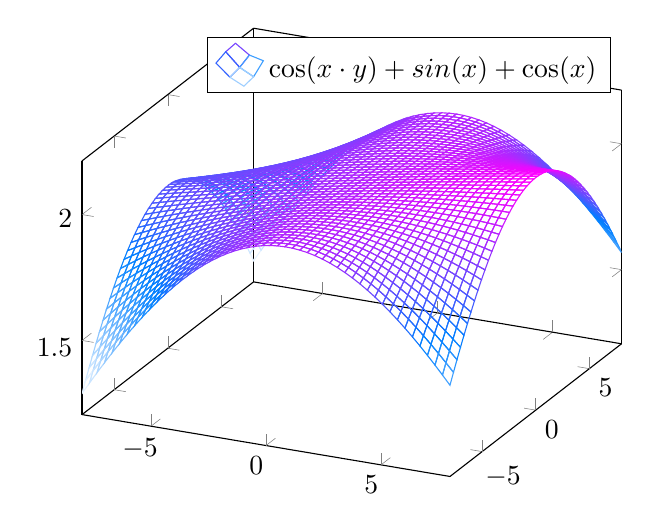
\begin{tikzpicture}
      \begin{axis}[
          % axis lines=center,
          colormap/cool,]
      \addplot3[
          mesh,
          samples=50,
          domain=-8:8,]
      {cos(x*y)+sin(x) + cos(x)};
      \addlegendentry{$\cos(x \cdot y) + sin(x) + \cos(x)$}
      \end{axis}
    \end{tikzpicture}
  \end{center}
\end{Beispiel}

%%% TODO:
%%% Hier bitte den Zusammenhang zwischen Matrizen, Polynomen und Multiniearabbildungen.


\section{Parameterintegrale}

Setup: $U \subseteq \R^n$ offen, $[a,b] \subseteq \R$, $a < b$ (also kompakt)
$$f : U \times [a,b] \to \R$$
Also als Form $f(x,t)$ mit $x$ als Parameter, und $t$ als Integrationsvariable.

Gesucht ist
$$F(x) = \int_a^b f(x,t) dt$$
mit $F: U \to \R$

\begin{Theorem}
  In dieser Situation gilt:
  $$f \text{ stetig } \Rightarrow F \text{ stetig}$$
  Falls für alle $k = 1,2,...,n$ die partielle Ableitung $\frac{\partial}{\partial x_k} f : U \times [a,b] \to \R$ existiert und stetig ist, dann ist $F$, gegeben durch
  $$F: U \to \R \quad F(x) = \int_a^b f(x,t) dt$$
  stetig differenzierbar und es gilt:
  $$\dfrac{\partial}{\partial x_k} F(x) = \int_a^b \dfrac{\partial}{\partial x_k} f(x,t) dt$$
\end{Theorem}

\begin{Beweis}
  Wir zeigen zunächst, dass $F$ stetig ist (bei $x_0 \in U$): Sei $\varepsilon > 0$, $r > 0$ klein genug, so dass der Ball $\overline{B(x_0, r)} \subseteq U$.

  Die Teilmenge $K = \overline{B(x_0, r)}$ von $U \times [a,b]$ ist kompakt (HB).

  Also ist $f|_K : K \to \R$ ist gleichmäßig stetig (weil $f$ stetig ist). Also
  $$\E \delta > 0 : |f(x_0, t) - f(x, t)| < \dfrac{\varepsilon}{b - a}$$
  für alle $x \in B(x_0, \delta)$ und für alle $t \in [a,b]$.

  Folgt: (für $x \in B(x_0,\delta)$)
  $$\begin{aligned}
    |F(x_0) - F(x)| & = \left|\int_a^b f(x_0,t) - f(x,t) dt \right| \\
    & \leq \int_a^b \underbrace{|f(x_0,t) - f(x,t)|}_{\leq \frac{\varepsilon}{b-a}} dt \\
    & \leq \varepsilon
  \end{aligned}$$
  Nun zeigen wir die Differenzierbarkeit von $F$ bei $x_0$:

  Wir wenden den Mittelwertsatz auf $h \mapsto f(x_0 + h \cdot s \cdot e_k \cdot t)$ für ein $s \in (-r,r)\backslash\{0\}$.

  Es existiert $\xi \in (0,1)$ mit
  $$\dfrac{\partial}{\partial x_k} f(x_0 + \xi, s \cdot e_k \cdot t) = \dfrac{f(x_0 + h \cdot s \cdot e_k \cdot t) - f(x_0, t)}{s}$$
  Da $\frac{\partial f}{\partial x_k}$ gleichmäßig stetig auf $K$ ist, existiert $\A \varepsilon > 0$ ein $\delta \in (0,r)$ mit
  $$\left| \dfrac{\partial}{\partial x_k} f(x_0, t) - \dfrac{\partial}{\partial x_k} f(x,t) \right| < \dfrac{\varepsilon}{b-a} \A x \in B, \A t \in [a,b]$$
  Wir zeigen nun, dass dieser Ausdruck, der Ableitung aus dem Satz entspricht, so wie $s \to 0$:
  $$\begin{aligned}
    & \left| \dfrac{F(x_0 + s\cdot e_k) - F(x_0)}{s} - \int_a^b \dfrac{\partial}{\partial x_k} f(x_0, t) dt \right| \\
    & = \left|\int_a^b \dfrac{f(x_0 + s \cdot e_k, t) - f(x_0)}{s} - \dfrac{\partial}{\partial x_k} f(x_0, t) dt \right| \\
    & = \left| \int_a^b \dfrac{\partial}{\partial x_k} f(x_0 + \xi \cdot e_k, t) - \dfrac{\partial}{\partial x_k} f(x_0,t) dt \right| \\
    & \leq \int_a^b \underbrace{\left| \dfrac{\partial}{\partial x_k} f(x_0 + \xi \cdot e_k, t) - \dfrac{\partial}{\partial x_k} f(x_0,t) \right|}_{< \frac{\varepsilon}{b-a} \text{ für } |s| < \delta} dt \\
    & \leq \varepsilon
  \end{aligned}$$
  Folgt: $\frac{\partial}{\partial x_k} F(x_0)$ existiert und ist gleich
  $$\int_a^b \dfrac{\partial}{\partial x_k} f(x_0, t) dt$$
  Die Stetigkeit folgt aus der anfänglichen Überlegung.
\end{Beweis}

\begin{Beispiel}[Bessel-Funktion]
  $$\mathcal{J}_n(x) = \dfrac{1}{\pi} \int_0^\pi \underbrace{\cos(x \cdot \sin(t) - nt)}_{f(x,t)} dt \quad n \in \Z$$
  (glatt in $x$ und $t$). Hier kann beispielsweise $x \in \C$.

  Für schwingende Körper, insbesondere Instrumente, gilt eine Differentialgleichung:
  $$x^2 u''(x) + x u'(x) + (x^2 - n^2)\cdot u(x) = 0 \qquad n \in \N$$

  $$\mathcal{J}_n'(x) = \dfrac{\partial \mathcal{J}_n(x)}{\partial x} = -\dfrac{1}{\pi} \int_0^\pi \sin(t) \cdot \sin(x \cdot \sin(t) - nt) dt$$
  $$\mathcal{J}_n''(x) = -\dfrac{1}{\pi}  \int_0^\pi \sin^2(t) \cdot \sin(x \cdot \sin(t) - nt) dt$$
  Jetz folgt
  $$\begin{aligned}
    x^2 \mathcal{J}_n''(x) + (x^2 - n^2)\mathcal{J}_n(x) & = \dfrac{1}{\pi} \int_0^\pi (\underbrace{-x^2\cdot \sin^2(t) + x^2}_{= x^2\cos^2(t)} - n^2)\cdot \cos(x \cdot \sin(t) -nt) dt \\
    & = \dfrac{1}{\pi} \int_0^\pi \underbrace{(x \cdot \cos(t) - n)}_{:= g} \underbrace{(x \cdot \cos(t) + n) \cdot \cos(x \cdot \sin(t) - nt)}_{=\frac{\partial}{\partial t} \sin(x\sin(t)-nt := f')} dt \\
    & = \dfrac{1}{\pi} \underbrace{\Big[(x \cos(t) + n)\sin(x \sin(t) - nt)\Big]_0^\pi}_{g \cdot f} \\
    & \quad + \dfrac{1}{\pi} \int_0^\pi \underbrace{(x \sin(t))\sin(x \sin(t) - nt) dt}_{g' \cdot f} \\
    & = 0 - x \cdot \mathcal{J}_n'(x)
  \end{aligned}$$
  Sei $j_{n,m} > 0$ die $m$-te Nullstelle von $\mathcal{J}_n(x)$. Es gilt: die Grundfrequenz $= j_{0,1}$.

  Das Bild für die Kreismembran hat dann für
  $$j_{n,m} \to \left\{ \begin{aligned}
    n & \text{ konzentrische Knotenlinien}\\
    m & \text{ Durchmesser}
  \end{aligned} \right.$$

  \begin{center}
    \includegraphics{./img/bessel_3d}

    Hier ist $n = 3$ und $m = 3$. Man erkennt, drei mal 3 konzentrische 'Hügel'.
  \end{center}

  Zur Berechnung der Nullstellen, betrachten wir die Taylor-Entwicklung
  $$\mathcal{J}_n(x) = \sum \limits_{m = 0}^\infty a_m \dfrac{x^m}{m!}$$
  $$\dfrac{\partial^m}{\partial x^m} \mathcal{J}_n(x) = \pm \dfrac{1}{\pi} \int_0^\pi \sin^m(t) {\sin \choose \cos} ( x \sin(t) - nt) dt$$
  Also
  $$a_m = \dfrac{\partial^m}{\partial x^m} \mathcal{J}_{n(0)} = \pm \dfrac{1}{\pi} \int_0^\pi \sin^m(t) \left\{ \begin{array}{c}\sin(nt) \\ \cos(nt) \end{array}\right. dt$$

  $$\mathcal{J}_n(x) = \sum \limits_{m = 0}^\infty \dfrac{(-1)m}{m!(m+n)!} \left(\dfrac{x}{2}\right)^{2m +2}$$

  \begin{center}
    \includegraphics{./img/bessel}

    Die $4$ ersten Bessel-Funktionen.
  \end{center}
\end{Beispiel}

\subsubsection{Glatte Funktionen konstruieren}

\begin{Beispiel}[Grundproblem]
  Wir haben $f : \R \to \R$, eine stetige Funktion. Wir möchten hierzu $\tilde{f} : \R \to \R$ finden/konstruieren mit
  \begin{enumerate}
    \item $\tilde{f}$ glatt
    \item $\tilde{f} - f$ beliebig klein: $|\tilde{f}(x) - f(x)| \leq \varepsilon \A x\in[a,b]$
  \end{enumerate}
\end{Beispiel}

\begin{Definition}[Träger]
  Sei $f: \R \to \R$ stetig. Der \textbf{Träger} von $f$ (support) ist
  $$\{x \in \R \mid f(x) \neq 0\} = supp(f)$$
  Die Funktion $f$ hat einen kompakten Träger genau dann, wenn
  $$f(x) = 0 \A x \in \R : |x| > R$$
  für ein $R >> 0$.
\end{Definition}

\begin{Definition}[Faltung]
  Sei $f: \R \to \R$ stetig und sei $\psi : \R \to \R$ ebenfalls stetig mit kompaktem Träger.

  Die \textbf{Faltung} (convolution) von $f$ mit $\psi$ ist die Funktion $\psi * f : \R \to \R$, definiert durch
  $$(\psi * f)(x) = \int_{-\infty}^\infty \psi(x-y)f(y)dy$$
  Das ist ein eigentliches Integral falls $\psi$ einen kompakten Träger hat,also falls $supp(\psi) \subseteq [-R,R]$:
  $$\int_{-R - |x|}^{R + |x|} \psi(x-y)f(y)dy$$
\end{Definition}

\begin{Theorem}
  $$\psi * f = f * \psi$$
\end{Theorem}

\begin{Beweis}
  $$\begin{aligned}
    (\psi * f)(x) & = \int_{-\infty}^\infty \psi(\underbrace{x-y}_{z})f(y)dy \\
    & = \int_{-\infty}^\infty \psi(z)f(x-z)dz \\
    & = (f*\psi) (x)
  \end{aligned}$$
\end{Beweis}

\begin{Bemerkung}
  Somit ist die Operation der Faltung kommutativ, assoziativ, linear in beiden Variablen (also bilinear).
\end{Bemerkung}

\begin{Theorem}
  Ist $f$ stetig und $\psi$ glatt, so ist $\psi * f$ glatt, und es gilt
  $$\dfrac{\partial}{\partial x} (\psi * f)(x) = \dfrac{\partial}{\partial x} \int_{-\infty}^\infty \psi(x-y)f(y)dy = \int_{-\infty}^\infty \psi'(x-y)f(y) dy = (\psi' * f)(x)$$
\end{Theorem}

\begin{Definition}[Glättungskern]
  Wir nennen eine Funktion $\psi: \R \to \R$ mit
  \begin{enumerate}
    \item $\psi$ ist glatt
    \item $supp(\psi) \subseteq [- \delta, \delta]$
    \item $\psi(x) \geq 0 \A x \in \R$
    \item $\int_{-\infty}^\infty \psi(x) dx = 1$
  \end{enumerate}
  \textbf{Glättungskern}.
\end{Definition}

\begin{Beispiel}
  $$\eta: \R \to \R \qquad \eta(x) = \left\{\begin{aligned} 0 & \text{ für } x \leq 0 \\ e^{-\frac{1}{x}} & \text{ für } x > 0\end{aligned}\right.$$
  ist glatt.
  \begin{center}
    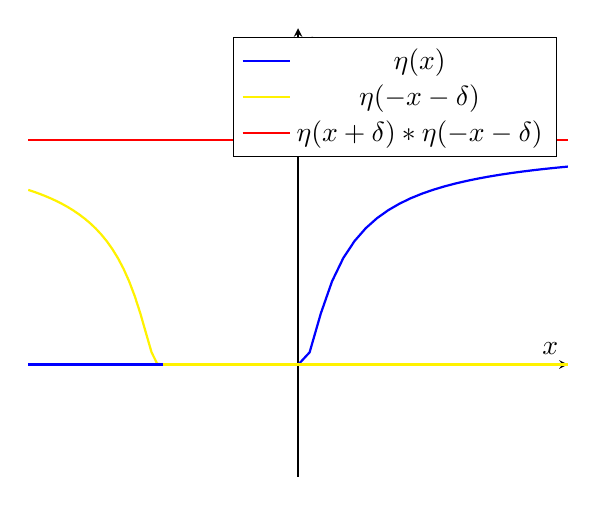
\begin{tikzpicture}
      \begin{axis}[
        domain=-8:8,
        ymin=-0.5,ymax=1.5,
        axis x line = center,
        xmajorticks=false,
        ticks=none,
        axis y line = center,
        xlabel={$x$},
        ylabel={$y$},
      ]

        \addplot[thick,blue,domain=0.01:8]{e^(-1/x)};
        \addlegendentry{$\eta(x)$}

        \addplot[thick,yellow,domain=-8:-4.01]{e^(-1/(-x-4))};
        \addlegendentry{$\eta(-x-\delta)$}


        \addplot[thick,red,domain=-8:8]{1};
        \addlegendentry{$\eta(x+ \delta)* \eta(-x -\delta)$}

        % Helpers
        \addplot[thick,blue,domain=-8:0.01]{0};
        \addplot[thick,yellow,domain=-4.01:8]{0};

      \end{axis}
    \end{tikzpicture}
  \end{center}
\end{Beispiel}

\begin{Bemerkung}[Warnung]
  Ist $\psi$ ein Glättungskern mit $supp(\psi) \subseteq [-\delta,\delta]$, dann ist $\psi' :=2 \psi(2x)$ ebenfalls ein Glättungskern mit $supp(\psi') \subseteq \left[-\dfrac{\delta}{2},\dfrac{\delta}{2}\right]$. Allgemein kann man bilden:
  $$\psi_n = 2^n \cdot \psi(2^n \cdot x) \qquad supp(\psi_n) \subseteq \left[-\dfrac{\delta}{2^n},\dfrac{\delta}{2^n}\right]$$
\end{Bemerkung}

Sei $f: \R \to \R$ stetig, $[a,b] \subseteq \R$, $a < b$. Sei $\varepsilon > 0$. Dann existiert ein $\delta > 0 $ mit
$$|y| < \delta \Rightarrow |f(x) - f(x-y)| < \varepsilon \A x\in [a,b]$$
Sei $\psi$ ein Glättungskern mit $supp(\psi) \subseteq [-\delta,\delta]$

Dann gilt für alle $x \in [a,b]$:
$$\begin{aligned}
  |(\psi * f)(x) - f(x)| & = \left|\int_{-\infty}^\infty \psi(x-y)f(y)dy - f(x)\right| \\
  & = \left|\int_{-\infty}^\infty \psi(x-y)f(y)dy - \int_{-\infty}^\infty \psi(y) f(x)dy \right| \\
  & = \left|\int_{-\infty}^\infty \psi(y)(f(x-y) - f(x)) dy \right| \\
  & \leq \int_{-\infty}^\infty |\psi(y)| \cdot \underbrace{|f(x-y) - f(x)|}_{\leq \varepsilon} dy \\
  & \leq \varepsilon
\end{aligned}$$
Die Annäherung an $\varepsilon$ ist möglich, wenn die Grenzen $-\infty ,  \infty$ zu $-\delta,\delta$ werden.

Setzen wir nun $f_n = \psi_n * f$ und $\psi_n(x) = 2^n \psi(2^n x)$, so konvergiert $(f_n)_{n = 0}^\infty$ gleichmäßig gegen $f$ auf jedem kompakten Intervall.


\section{Wegintegrale}
Setup: $U \subseteq \R^n$ offen. $\gamma : [a,b] \to U$ stetig differenzierbar.

Sei $\gamma(t)$ die Position zur Zeit $t \in [a,b]$ und $\gamma'(t)$ der Geschwindigkeitsvektor $\in \R^n$. Also ist $||\gamma'(t)||$ die Geschwindigkeit.
$$\int_a^b ||\gamma'(t)|| dt = \text{ Länge von } \gamma$$
ist $f : U \to \R$ eine stetige Funktion,
$$\int_a^b f(\gamma(t)) \cdot ||\gamma'(t)|| dt$$
Ist $\gamma$ stückweise differenzierbar
$$a \leq t_1 < t_2 < ... < t_n \leq b : \gamma|_{[t_i,t_{i+1}]} \text{ stetig differenzierbar}$$
dann ergeben die obigen Begriffen weiterhin Sinn.

\begin{Definition}[Vektorfeld]
  Sei $U \subseteq \R^n$ offen. Ein (stetiges, differenzierbares, glattes [insert attribute here]) \textbf{Vektorfeld} auf $U$ ist eine (stetige, differenzierbare, glatte [insert same attribute]) Funktion $F:U \to \R^n$.

  Sei $\gamma:[a,b] \to U$ stetig differenzierbar und $F: U \to \R^n$ ein stetiges Vektorfeld.
  $$\int_\gamma F dt = \int_a^b <F(\gamma(t)),\gamma'(t)> dt$$
  \textbf{Terminologie:}

  Eine stetige, orientierungserhaltende Reparameterisierung von $\gamma : [a,b] \to U$ ist eine Verknüpfung
  $$\gamma \circ \psi \quad \text{mit} \quad [c,d] \stackrel{\psi}{\longrightarrow} [a,b] \stackrel{\gamma}{\longrightarrow} U$$
  Mit $\psi$ stetig, $\psi(c) = a$, $\psi(d) = b$.
\end{Definition}

\begin{Theorem}[Arbeitsintegral]
  Das \textbf{Arbeitsintegral} $(x)$ ändert sich nicht durch orientierungserhaltende Reparameterisierungen.
\end{Theorem}

\begin{Beweis}
  $$\begin{aligned}
    \int_{\gamma \circ \psi} F dt & = \int_c^d <F(\gamma(\psi(t))), \underbrace{(\gamma \circ \psi)'(t)}_{\gamma'(\psi(t))\psi'(t)}> dt \\
    & = \int_c^d <F(\gamma(\psi(t))), (\gamma(\psi))(t)> \cdot \psi'(t) dt \\
    & = \int_a^b <F(\gamma(s)),\gamma'(s)> ds
  \end{aligned}$$
\end{Beweis}

\begin{Definition}[Potential]
  Sei $U \subseteq \R^n$, $F : U \to \R^n$ ein stetiges Vektorfeld und $\gamma:[a,b] \to U$ stückweise stetig differenzierbar (also an endlich vielen Punkten nicht differenzierbar.)
  $$\int_\gamma F dt \sim \int \vec{F} d\vec{s} \text{ bedeutet } \int_a^b<F(\gamma(t)),\gamma(t)> dt$$

  Eine Funktion $f:U\to \R$ heißt \textbf{Potential} von $F$, falls
  $$F = grad(f)$$
  Ist $f$ ein Potential, so ist auch $f+c$ für $c \in \R$. Ist $U$ zusammenhängend, so ist jedes weitere Potential von $F$ derselben Form.
\end{Definition}

\begin{Theorem}
  Sei $f$ ein Potential für $F$. Dann gilt
  $$\int_\gamma F dt = f(\gamma(1)) - f(\gamma(0))$$
  für jeden differenzierbaren Pfad $\gamma [0,1] \to U$.

  Dies entspricht der aus der Physik bereits bekannten Wegunabhängigeit für konservative Felder.
\end{Theorem}

\begin{Beweis}
  Bemerke zunächst: $F(x) = grad(f)(x) = Df(x)$ also $\Rightarrow <grad(f)(x),v> = Df(x)(v)$. Nun gilt
  $$\begin{aligned}
    \int_\gamma F dt & = \int_0^1 <grad(f)(\gamma(t)),\gamma'(t)> dt \\
    & = \int_0^1 Df(\gamma(t)) \cdot \gamma'(t) dt \\
    & = \int_0^1 (f \circ \gamma)' dt \\
    & = f(\gamma(1)) - f(\gamma(0))
  \end{aligned}$$
\end{Beweis}

\begin{Beispiel}
  $$U = \R^2 \quad F(x,y) = (-y,x)$$
  \begin{center}
    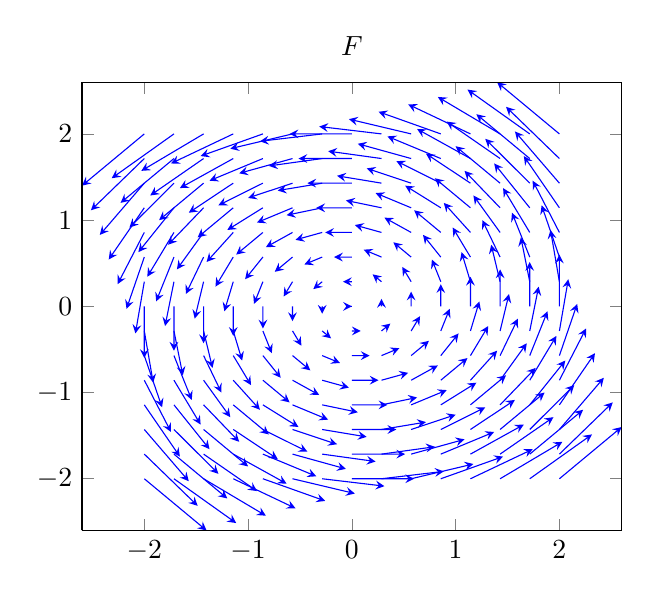
\begin{tikzpicture}
      \begin{axis}[
          title={$F$},
          domain=-2:2,
          view={0}{90},
          axis background/.style={fill=white},
      ]
          \addplot3[blue,
              quiver={
               u={-y},
               v={x},
               scale arrows=0.3,
              },
              -stealth,samples=15]
                  {0};
      \end{axis}
    \end{tikzpicture}
  \end{center}


  Sei nun $\gamma: [0,1] \to U$ mit $\gamma(t) = (t,t)$ und betrachte insbesondere den Pfad von $(0,0)$ nach $(1,0)$ nach $(1,1)$. Es gilt
  $$\int_\gamma F dt = \int_0^1 \underbrace{<(-t,t),(1,1)>}_{0} dt = 0$$
  was nicht besonders verwunderlich ist.

  Betrachte nun $\gamma(t) = \left\{\begin{aligned}
    (2t,0) & 0 \leq t \leq \frac{1}{2} \\
    (1, 2t-1) & \frac{1}{2} \leq t \leq 1
  \end{aligned}\right.$
  $$\begin{aligned}
    \int_\gamma F dt & = \int_0^{\frac{1}{2}} \underbrace{<(0,2t),(2,0)>}_{0} dt + \int_{\frac{1}{2}}^1 \underbrace{<(-2t+1,1),(0,2)>}_{2} dt \\
    &= 1
  \end{aligned}$$
  Da die Beiden Arbeitsintegrale nicht übereinstimmen gilt: $F$ hat \textbf{kein} Potential.
\end{Beispiel}

\begin{Definition}[Konservative Vektorfelder]
  Ein stetiges Vektorfeld $F:U \to \R^n$ nennen wir \textbf{konservativ}, falls für alle Wege $\gamma,\varphi :[0,1] \to U$ mit $\gamma(0) = \varphi(0)$ und $\gamma(1) = \varphi(1)$ gilt
  $$\int_\gamma F dt = \int_\phi F dt$$
\end{Definition}

\begin{Theorem}
  Sei $U \subseteq \R^n$ offen und zusammenhängend. Sei $F: U \to \R^n$ ein stetiges Vektorfeld.
  $$F \text{ ist konservativ } \Leftrightarrow F \text{ hat ein Potential}$$
\end{Theorem}

\begin{Beweis}
  Die eine Richtung wurde bereits oben gezeigt.

  Sei nun $F$ konservativ. Wähle $x_0 \in U$ und definiere
  $$f(x) = \int_{\gamma (x)} F dt \qquad f:U\to \R^n$$
  Für einen Pfad $\gamma:[0,1] \to U$ mit $\gamma(0) = x_0$ und $\gamma(1) = x$
  \incfig{pfad_beweis_konservativ}
  \underline{Behauptung:} $grad(f) = F$, also $\dfrac{\partial}{\partial x_k} f(x) = F_k(x) = <F(x),e_k> \A x \in U$
  $$\begin{aligned}
    f(x + h \cdot e_k) - f(x) & = \\
  \end{aligned}$$
  Wähle nun einen Pfad $\varphi$ von $x$ nach $x + h \cdot e_k$, also $\varphi(t) = h + t \cdot h \cdot e_k$.
  Nun gilt:
  $$\begin{aligned}
    \limh \dfrac{f(x + h \cdot e_k) - f(x)}{h} & = \limh \dfrac{1}{h} \int_0^1 <F(\varphi(t)),\varphi'(t)> dt \\
    & = \limh \int_0^1 <F(x + th e_k),\not h \cdot e_k> dt \\
    & = \int_0^1 <F(x),e_k> dt \\
    & = <F(x),e_k>
  \end{aligned}$$
\end{Beweis}

\begin{Korollar}[Integrabilitätsbedingung]
  Es sei $F : U \to \R^n$ ein konservatives Vektorfeld der Klass $\mathcal{C}^1$. Dann gilt
  $$\dfrac{\partial}{\partial x_k} F_j(x) = \dfrac{\partial}{\partial x_j} F_k(x)$$
\end{Korollar}
\begin{Beweis}
$$\dfrac{\partial}{\partial x_k} F_j(x)  = \dfrac{\partial}{\partial x_k} \dfrac{\partial}{\partial x_j} f(x)$$
$$= \text{ \small (Satz von Schwarz)}$$
$$\dfrac{\partial}{\partial x_j} F_k(x)  = \dfrac{\partial}{\partial x_j} \dfrac{\partial}{\partial x_k} f(x)$$
\end{Beweis}

\begin{Beispiel}
  Sei $U = \R^2$ und $F : U \to \R^2$ das Vektorfeld gegeben durch
  $$F(x,y) = (e^x, \sin(y))$$
  Existiert jetzt ein $f: \R^2 \to \R^2$ mit
  $$\dfrac{\partial f}{\partial x} = e^x \quad \dfrac{\partial f}{\partial y} = \sin(y)$$
  ? Ja, offensichtlich
  $$f(x) = e^x - \cos(y)$$
  Und man sieht, dass die Integrabilitätsbedingung gilt.
\end{Beispiel}

\begin{Beispiel}
  Sei $U = \R^2$ und $F : U \to \R^2$ das Vektorfeld gegeben durch
  $$F(x,y) = \left(yx^2, \sin\left(\dfrac{1}{1 + x^2 + y^2}\right)\right)$$
  \begin{itemize}
    \item $\dfrac{\partial }{\partial x} f(x,y) = yx^2$
    \item $\dfrac{\partial }{\partial y} f(x,y) = \sin\left(\dfrac{1}{1 + x^2 + y^2}\right)$
  \end{itemize}
  Notwendig hierfür ist die Integrabilitätsbedingung:
  $$f(x,y) = \int_\gamma F dt \text{ mit } \gamma(0)=(0,0) \quad \gamma(1)=(x,y)$$
  Prüfe
  $$\dfrac{\partial}{\partial y} F_1(x,y) = x^2$$
  $$\dfrac{\partial}{\partial x} F_2(x,y) = \dfrac{-2 \cdot 2x}{1 + x^2 + y^2}\cos\left(\dfrac{1}{1 + x^2 + y^2}\right)$$
  Also existiert keine Lösung.
\end{Beispiel}

\begin{Theorem}[Globaler Integrationssatz (Beispiel)]
  Ist $F: U \to \R^n$ von Klasse $\mathcal{C}^2$ und sind $\gamma, \phi : [0,1] \to U$ Pfade mit $\gamma(0) = \varphi(0)$ und $\gamma(1) = \varphi(1)$.

  Erfüllt $F$ die Integrabilitätsbedingung, so gilt
  $$\int_\gamma F dt = \int_\varphi F dt \Leftrightarrow \varphi \text{ ist homotop zu } \gamma$$
\end{Theorem}

\begin{Korollar}
  Ist $U$ einfach zusammenhängend, dann ist $F$ \textbf{konservativ}.
\end{Korollar}

\begin{Lemma}
  Sei $U \subseteq \R^n$ konvex und $F:U \to \R$ ein Vektorfekd der Klasse $\mathcal{C}^1$ mit der Integrabilitätsbedingung. Dann ist $F$ konservativ.
\end{Lemma}

\begin{Beweis}[des Lemmas]
  Nehme oBdA an: $x_0 \equiv 0 \in \R^n$. Wir definieren eine Funktion $f: U \to \R$ durch
  $$f(x) = \int_0^1 <F(t\cdot x),x> dt$$
  (also über einen Pfad, in diesem Fall die gerade Linie)

  Wir wollen nun zeigen, dass $f$ ein Potential für $F$ ist. Hierzu berechnen wir vorbereitend:
  $$\begin{aligned}
    \partial_h F_j (x) = DF_j(x)(h) & = <grad[F_j(x)],h> \quad h \in \R^n \\
    & = \sum \limits_{k=1}^n \partial_k F_j(x)\cdot h_k \\
    & = \sum \limits_{k=1}^n \partial_j F_k(x)\cdot h_k
  \end{aligned}$$
  Die letzte Gleichheit gilt dank der Integrabilitätsbedingung.

  Es gilt:
  $$\begin{aligned}
    \partial_j f(x) & = \dfrac{\partial}{\partial x_j} \int_0^1 \sum \limits_{k=1}^n F_k (t\cdot x) \cdot x_k dt \\
    & =  \int_0^1 \sum \limits_{k=1}^n \dfrac{\partial}{\partial x_j}  F_k (t\cdot x) \cdot x_k dt \\
    & = \int_0^1 \sum \limits_{k=1}^n (t \cdot \partial_j F_k(t\cdot x) \cdot x_k) + F_j(t \cdot x) dt \\
    & \stackrel{s.o.}{=} \int_0^1 t \cdot \underbrace{\partial_x F_j(t \cdot x)}_{\frac{\partial}{\partial t} F_j (t \cdot x)} + F_j(t \cdot x) dt\\
    & = \int_0^1 t \cdot \partial_x F_j(t \cdot x) dt + \int_0^1 F_j(t \cdot x) dt \\
    & = \Big[t \cdot F_j(t \cdot x)\Big]_0^1 - \int_0^1 F_j(t \cdot x) dt + \int_0^1 F_j(t \cdot x) dt \\
    & = F_j(x)
  \end{aligned}$$
  $$\Rightarrow grad(f) = F$$
\end{Beweis}

\subsubsection{Vorbereitung des Beweises des globalen Integrationssatzes}

\begin{Definition}[Zurückgezogenes Vektorfeld]
  Sei $\varphi: V \to U$ von Klasse $\mathcal{C}^1$ mit $V \subseteq \R^m$ offen, $U \subseteq \R^n$ offen.
  $$\varphi^* :\{\text{stetige VF auf $U$}\} \to \{\text{stetige VF auf $V$}\}$$
  sei gegeben durch
  $$(\varphi^* F)(x) = \sum \limits_{k = 1}^m \underbrace{<\partial_k \varphi(x) , F(\varphi(x))>}_{k\text{-te Komponente von }\varphi^* F} \cdot e_k \A x \in V, \A \text{Vektorfelder } F: U \to \R^n$$
  $\varphi^*$ ist das \textbf{zurückgezogen Vektorfeld} zu $\varphi$
\end{Definition}

\begin{Theorem}
  Sei $\varphi^*$ wie in der obigen Definition.
  \begin{enumerate}
    \item $\varphi^*$ ist linear.
    \item $\varphi^*$ ist funktioral: Für
      $$W \stackrel{\psi}{\to} V \stackrel{\varphi}{\to} U$$
      gilt: $(\varphi \circ \psi)^* = \psi^* \circ \varphi^*$
      \begin{Bemerkung}
        Also gilt insbesondere: $(id \circ \varphi)^* = \varphi^*$
      \end{Bemerkung}
    \item Sei $\gamma: [0,1] \to V$ stetig differenzierbar und $F: U \to \R^n$ stetig
      $$\int_\gamma \varphi^* F dt = \int_{\varphi \circ \gamma} F dt$$
    \item Ist $F$ von Klasse $\mathcal{C}^p$, $\varphi$ von Klasse $\mathcal{C}^{p+1}$, so ist $\varphi^* F$ von Klasse $\mathcal{C}^p$
    \item Ist $F$von Klasse $\mathcal{C}^1$, $\varphi$ von Klasse $\mathcal{C}^2$. Falls $F$ die Integrabilitätsbedingung, so erfüllt $\varphi^* F$ sie ebenfalls.
  \end{enumerate}
\end{Theorem}

\begin{Beweis}
  Siehe Skript, insbesondere bis Punkt $3$.
\end{Beweis}

Nun beweisen wir endlich den globalen Integrationssatz (also das eine Beispiel von ihm).

\begin{Beweis}[Illegal]
  Setup wie gewohnt: $U \subseteq \R^n$, $f : U \to \R^n$ von Klasse $\mathcal{C}^1$ erfüllt die Integrabilitätsbedingung.

  Seien $\gamma_0, \gamma_1 : [0,1] \to U$ stückweise stetig differenzierbar mit $x_0 = \gamma_0(0) = \gamma_1(0)$ und $x_1 = \gamma_0(1) = \gamma_1(1)$ und $\gamma_0 \stackrel{htp}{\backsimeq} \gamma_1$.
  Also existiert eine Homotopie von $\gamma_0$ nach $\gamma_1$:
  $$\begin{array}{c c c}
    H:[0,1]^2 & \to & U \\
    H(0,t) = \gamma_0(t) & & H(1,t) = \gamma_1(t) \\
    H(s,t) = X_0 & & H(s,1) = x_1
  \end{array}$$
  $$\begin{aligned}
    \int_{\gamma_0} F dt & = \int_{H \circ \varphi_0} F dt \\
    & = \int_{\varphi_0} H^* F dt \quad \text{erfüllt laut 5) die Integrabilitätsbedingung} \\
    (Lemma) & = \int_{\varphi_1} H^* F dt \\
    & = \int_{H \circ \varphi_1} F dt \\
    & = \int_{\gamma_1} F dt
  \end{aligned}$$
  Leider falsch, denn:
  \begin{enumerate}
    \item Wir betrachten einen nicht-offenen Definitionsbereich von $H$: $[0,1]^2$ hier sind Differenzierbarkeit und Pfade am Rand noch gar nicht definiert worden.
    \item $H$ ist stetig, aber nicht $\in \mathcal{C}^2$
  \end{enumerate}
\end{Beweis}

\begin{Beweis}[Probleme behoben]
  \incfig{globaler_integrationssatz}
  \begin{enumerate}
    \item Wir dehnen den Definitionsbereich von $H$ auf $\R^2$ aus: $H: \R^2 \to U$ ist gleichmäßig stetig und hat ein kompaktes Bild.
    \item Für $N \in \N$ konstruieren wir $H_N: \R^2 \to U$ mit ($N \to \infty$)
    $$||H - H_N||_\infty \longrightarrow 0$$
    $H_N$ von Klasse $\mathcal{C}^\infty$.

    Wähle einen Glättunfskern $\eta$ mit $supp(\eta) \subseteq (-1,1)$
    $$\eta_N(u) = 2^N \eta(2^{-N} u)$$
    Benutze diesen Kern um $H$ zu glätten:
    $$H_N(x,y) \int_{-\infty}^\infty \eta_N(v) \cdot \int_{-\infty}^\infty \eta_N(u)H(x-u,y)du dv$$
    (Glättung nach beiden Variablen).

    $||H_N - H||_\infty \to 0$ weil $H$ gleichmäßig stetig.

    Jetzt gilt:
    $$\int_{H_N \circ \gamma_0} F dt = \int_{H_N \circ \gamma_1} F dt$$
    Hier haben wir nur eine Annäherung an $\gamma_0$ und $\gamma_1$. Es gilt aber
    $$H_N \circ \gamma_0 = \int_0^1 <F(Hn(\varphi_0(t))),(H_n \circ \varphi)'(t)> dt \longrightarrow \int_{\gamma_0} F dt$$
    (für $N \to \infty$)
    
    Die Grenzwertbildung ist mit dem Integral vertauschbar wegen der gleichmäßigen Stetigkeit. Man geht analog für $\gamma_1$ vor.
  \end{enumerate}
\end{Beweis}

\end{document}
